\chapter{THE PACKET PIPELINE PROCESSING MODEL} \label{pipeline_model}

The Steve programming language uses a pipeline model for processing packets. A pipeline is a composition of two types of processing stages: decoding stages and table matching stages. Each stage performs a set of operations on a packet, known as actions, and decides where to move the packet next based on certain conditions that the packet meets. A packet can be moved to another processing stage or it can be sent out of the pipeline.

The pipeline is thus a state machine. Each processing stage denotes a state in the machine. Each state has a set of conditions which, when met, causes the packet to transition states. This can be represented as a graph where each processing stage is a node on the graph and each state transition is an edge connecting stages.

\section{Decoding Stage}

When a packet is received, it is simply a chunk of raw, uninterpreted data. Before a packet can be processed and routed, its headers and fields must be decoded and extracted so that meaningful decisions can be made about what to do with the packet. The decoding stage is responsible for ensuring this happens.

Steve allows for programmers to specify \textit{how} and \textit{which} fields are extracted from packet headers. In other paradigms, the \textit{entire} packet is decoded from start to finish; all headers and all fields are extracted, then all fields are saved. This is what is considered a \textbf{full decode}. After this full decode, the decision making process on the packet begins using those saved fields. However, this method is inherently inefficient. Only certain fields and headers within a packet are ever really needed during the routing process. To compound this, different switches may care about different subsets of fields within a given packet. Decoding all of these fields does not make sense when only a smaller subset is ever necessary. 

Full decodes waste valuable processing time. Efficiency is important when dealing with networking equipment which has to processes between 10Gbps to 40Gbps. Decoding fields which are not needed is equivalent to wasting clock cycles on the CPU. This could translate to drastically slower performance.

This inherent inefficiency is why Steve proposes the idea of a \textit{partial decode}. Unlike other similar languages, Steve is designed to allow programmers to specify the extraction of only specific fields rather than an entire header. Though the specification may be verbose in some cases, it makes programmers think very carefully about which fields they need and which fields they do not.

Additionally, Steve proposes that not all headers need to be decoded. For example, if a networking application only needs to forward using MAC addresses, there is no reason to waste time extracting fields from IPv4 or IPv6 headers, and so on.

\subsection{Packet Context}

As a packet moves between stages, information such as the position and length of fields and headers must be saved so that they can be recovered when needed in later stages of the pipeline. Remember, tables classify packets and perform actions on them based on the values of extracted fields. To save this information, Steve applications uses a data structure called the packet \textbf{context}. Specifically, a Steve context saves the following data:

\begin{itemize}
\item The logical and physical port the packet arrived on.
\item The length of the packet frame.
\item A tunnel identifier.
\item The offset and length of a field in the packet.
\item The offset of a header in the packet.
\end{itemize}

In order to support saving the extracted fields and headers, they get saved in \textbf{binding environments} contained within the context. The term \textbf{environment} refers to a mapping of names (in this case field and header names) to their storage location during runtime \cite{compilers1}. The mapping of those storage locations to the values held there is known as \textbf{state}. There is a binding environment for fields and headers respectively.

Figure \ref{fg:ContextEnv} depicts the binding environment. The field environment is used to map fields with offset-length pairs where that field can be found in the packet. The packet header environment similarly maps headers with the offsets where that header can be found in the packet. These mappings are known as \textit{bindings}.

Since any given packet can contain one or more of any field or header with the same name, the environments maintain a stack for every field and header. These stacks are what are called \textit{binding stacks}. By extension, this means an environment is actually a mapping of fields to binding stacks. When the value of a field is needed, the topmost binding on the binding stack shall be used to recover the state of that field.

The implementation of environments in Steve is a fixed-sized array where each element in the array is a fixed-sized binding stack. Each index in the array represents a unique field or header name extracted by the Steve application. The compiler is responsible for associating all unique fields extracted during the decoding stage to unique integer indices into the array. The same is done for all unique headers. This provides constant time lookup of field bindings without the overhead of hashing found in environments which use complex name mappings.

\begin{figure}[ht]
\centering
		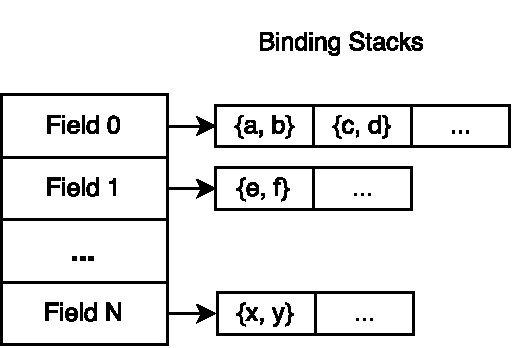
\includegraphics[scale=0.75]{context}
\caption{The binding environment inside a context used to store the length and offset of fields, or the offset of headers. On the left, fields one through sixteen represent the fields that can be extracted. Each field maintains a binding list (stack). Each element in the binding list is a binding which stores the offset and length where each instance of that field can be found in the packet. }
\label{fg:ContextEnv}
\end{figure}

Figure \ref{fg:ContextEnvWorking} demonstrates how data is stored in the context as it is being decoded. The example is a packet which contains an encapsulated IPv4 header commonly used in IP tunneling. In the ethernet decoding stage which extract the \texttt{src}, \texttt{dst}, and \texttt{type} field are extracted and stored in the context. Next we determine that IPv4 follows based on the \texttt{type} field. We extract IPv4 \texttt{dst} and \texttt{protocol}. The \texttt{protocol} field tells us we have another IPv4 header after the current one. We move to decode that and once again we extract IPv4 \texttt{dst} and \texttt{protocol}. Note how the new values of IPv4 are pushed on top of the binding stack. Any further usage of those fields will use the latest values extracted for those fields. Keep in mind that this means any usage of the first set of IPv4 \texttt{dst} and \texttt{protocol} must occur before the decoding of the second IPv4 header.

\section{Table Stage}

Table stages handle matching the extracted fields, i.e. classification, and perform a sequence of desired actions on like-classified packets. Tables used in the Steve runtime use similar semantics to the OpenFlow specification \cite{openflow_spec}. A table stage is comprised of two parts: the table and a set of unique flow entries.

A table specifies what fields from what headers are to be used for matching. For example, a table which handles forwarding on Layer 2 of the OSI stack may choose to match on the \texttt{src} and \texttt{type} fields in an ethernet header. A table used for IP routing may choose to match on the \texttt{src} and \texttt{protocol} fields. 

Tables are not obligated to match on fields from a single header. A table can match on any set of fields previously extracted.

A table contains a set of \textbf{flow entries}. A flow entry is defined by a table-unique key, a priority, and a sequence of actions that are to be applied to packets. An \textbf{action} can transition a packet to another stage, modify it, forward it, delete it, add flow entries, or remove flow entries. Further details can be found in \ref{action_semantics}.

When a packet reaches a table matching stage, the value of the fields that the table matches against are recovered from the context. These values become sub-keys which are merged together into a single key for the packet. From there, the table finds all flow entries whose key matches the packet's key. The packet with the highest priority is selected and its sequence of actions are applied to the packet.

If no such flow entry matches the packet's key, the \textbf{miss case} flow entry is applied to the packet instead. By default, a miss in a table results in the packet being dropped. With Steve, a programmer can also specify a user-defined miss case. Miss cases always have the lowest possible priority amongst flow entries and each sub-key can be considered a wildcard value.


\section{Pipeline Composition}

Kinds of processing stages can be interleaved together in any order within the pipeline. This means that Steve is capable of supporting different packet processing paradigms found in other research such as POF and P4. With the Steve pipeline specification language a user can specify that a pipeline does:

\begin{enumerate}
\item \textbf{A full decode of the packet followed by a sequence of tables.} Packets coming to the pipeline have all necessary headers and fields are decoded and saved in the runtime context first. The packet is then dispatched to the first table in the pipeline. From there, matched flows within the tables dictate which table the packet is sent to next or which port the packet is forwarded to.
\item \textbf{A chain of partial decodes and table lookups.} Packets coming to the pipeline get partially decoded and dispatched to a table. The flow within that table could carry the packet to another table, another decoder, or forward it out of the network. The pipeline in this case in a chain of alternating sequences of decoding stages and table matching stages.
\item \textbf{Only decodes.} In some special cases, it may not even be necessary to go to a table matching stage. It may be possible to make a decision about the packet’s ultimate destination immediately upon evaluating a certain field within the packet using a simple conditional statement (if-statement, if-else statement, etc). Therefore, decoding stages also support the range of actions supported by flow entries, which can include outputting packets to a port or dropping it.
\end{enumerate}

Upon entering the pipeline, a packet must first go through at least one decoding stage before moving to the next processing stage. From there, the packet flows from one stage of the pipeline to the next. With each stage, certain conditions are evaluated which will determine where the packet must flow next. Finally, the packet will exit the pipeline either through a port(s) or by being dropped and discarded.

